\documentclass[methods.tex]{subfiles}
 
\begin{document}

\chapter{Long-range dependence}

\section{What is long-range dependence?}

\paragraph{Time series:} Any sequence of observations associated with an ordered independent variable $t$. For the analyses carried out in this report, we assume that the time series is defined essentially over a range of integers (usually $t = 0 , 1 , ... , N - 1$, where $N$ denotes the number of values in the time series).

\paragraph{Random variable:} A real-valued random variable is a function, or mapping, from the sample space of possible outcomes of a random experiment to the real line.

\paragraph{Stochastic process:} A discrete parameter real-valued stochastic process $\left\{ X_t : t = ... , -1 , 0 , 1 , ... \right\}$ is a sequence of random variables indexed over the integers. A process such as $\left\{ X_t \right\}$ can serve as a stochastic model for a sequence of observations of some physical phenomenon. We assume that these observations are recorded at a sampling interval of $\Delta t$.

\paragraph{Stationarity:} The process $\left\{ X_t \right\} $ is said to be (second order) stationary if:
\begin{enumerate}
\item $E \left\{ X_t \right\} = \mu_X$ for all integers $t$ (i.e. $\mu_X$ does not depend on $t$).
\item $cov \left\{ X_t , X_{t + \tau} \right\} = s_{X , \tau}$ for all integers $t$ and $\tau$ (i.e. $s_{X , \tau}$ depends only on $\tau$ and does not depend on $t$).
\end{enumerate}

\paragraph{Autocovariance sequence (ACVS):} The sequence $\left\{ s_{X , \tau} : \tau = ... , -1 , 0 , 1 , ... \right\}$. The autocorrelation sequence (ACS) is $\rho_{X , \tau} = s_{X , \tau } / s_{X , 0}$.

\paragraph{Spectral density function (SDF), or power spectrum:} $S_X \left( f \right) = \Delta t \sum_{\tau = - \infty}^{\infty} s_{X , \tau} e^{- i 2 \pi f \tau \Delta t} \text{ for } \left| f \right| \leq f_N = \frac{1}{2 \Delta t}$, that is $S_X \left( . \right)$ is the Fourier transform of $\left\{ s_{X , \tau} \right\}$.

\paragraph{Stationary long memory process:} $\left\{ X_t \right\}$ is a stationary long memory process if there exist constants $\alpha$ and $C_S$ satisfying $ -1 < \alpha < 0$ and $C_S > 0$ such that:

\begin{equation}
\lim_{f \to 0} \frac{S_X \left( f \right)}{C_S \left| f \right| ^{\alpha}} = 1 \text{ that is } \log \left( S_X \left( f \right) \right) = \beta + \alpha \log \left( f \right)
\end{equation}

\newpage

\section{Long-range dependence in low-frequency earthquake catalogs?}

Episodic Tremor and Slip (ETS) is a phenomenon that takes place mostly in subduction zones, when a geodetically detected slow slip event occurs concurrently with tectonic tremor. Tremor is a long (several seconds to many minutes), low amplitude seismic signal, with emergent onsets, and an absence of clear impulsive phases. Their occurrence is correlated temporally and spatially with slow slip events on the subduction zone interface. At least a portion of the tremor is made of small low-frequency earthquakes (LFEs). LFEs group into families, or clusters of LFEs that repeat on small $\approx$ 1 km\textsuperscript{2} patches on the plate interface. \\

For a given LFE family, we can obtain from the seismic data an event catalog that gives the exact timing (and sometimes the magnitude) of each small earthquake occurring on this given small patch. We can then construct a time series by counting the number of events occurring in every time windows of a given duration. For example, Frank \textit{et al.} (2016) translated their LFE catalog from Guerrero, Mexico, into a discrete event count signal with regular time steps of 1 min, binning each cataloged event into the time step during which it is observed. They then computed an autocorrelation function for this time series. Finally, they computed the Fourier spectrum of the event count autocorrelation (see Figure 8.1). \\

\begin{center}
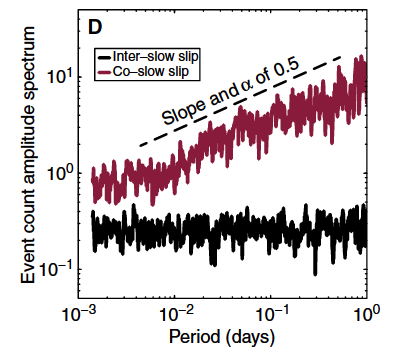
\includegraphics[width=300pt, trim={0cm 0cm 0cm 0cm},clip]{Figures/longrange/Frank_et_al_2016_Fig2D.png}
\captionsetup{type=figure}
\captionof{figure}{Figure 2D of Frank \textit{et al.} (2016). We have $\log \left( S_X \left( f \right) \right) = \beta + \alpha \log \left( f \right)$ with $\alpha = - 0.5$ where $S_X$ is the spectral density function (SDF), or power spectrum, and $f$ is the frequency.}
\end{center}

I have taken a family of LFEs recorded in the Olympic Peninsula, Washington (catalog from Sweet \textit{et al.}, 2014) and applied several estimators from Taqqu and Teverovsky (1998) to measure the intensity of long-range dependence in the event count time series. \\

Let us define a time series $X_i$, of length $N$. We define the corresponding aggregated series:

\begin{equation}
X^{\left( m \right)} \left( k \right) = \frac{1}{m} \sum_{i = \left( k - 1 \right) m + 1}^{k m} X_i \text{, } k = 1 , 2 , ... , \left[ \frac{N}{m} \right]
\end{equation}

The first absolute moment of the time series is then:

\begin{equation}
AM^{\left( m \right)} = \frac{m}{N} \sum_{k = 1}^{\frac{N}{m}} \left| X^{\left( m \right)} \left( k \right) - \bar{X} \right|
\end{equation}

and $AM^{\left( m \right)}$ behaves as $m^{H - 1}$, where $H$ is the Hurst parameter. The result of the corresponding linear regression can be seen in Figure 8.2.

\begin{center}
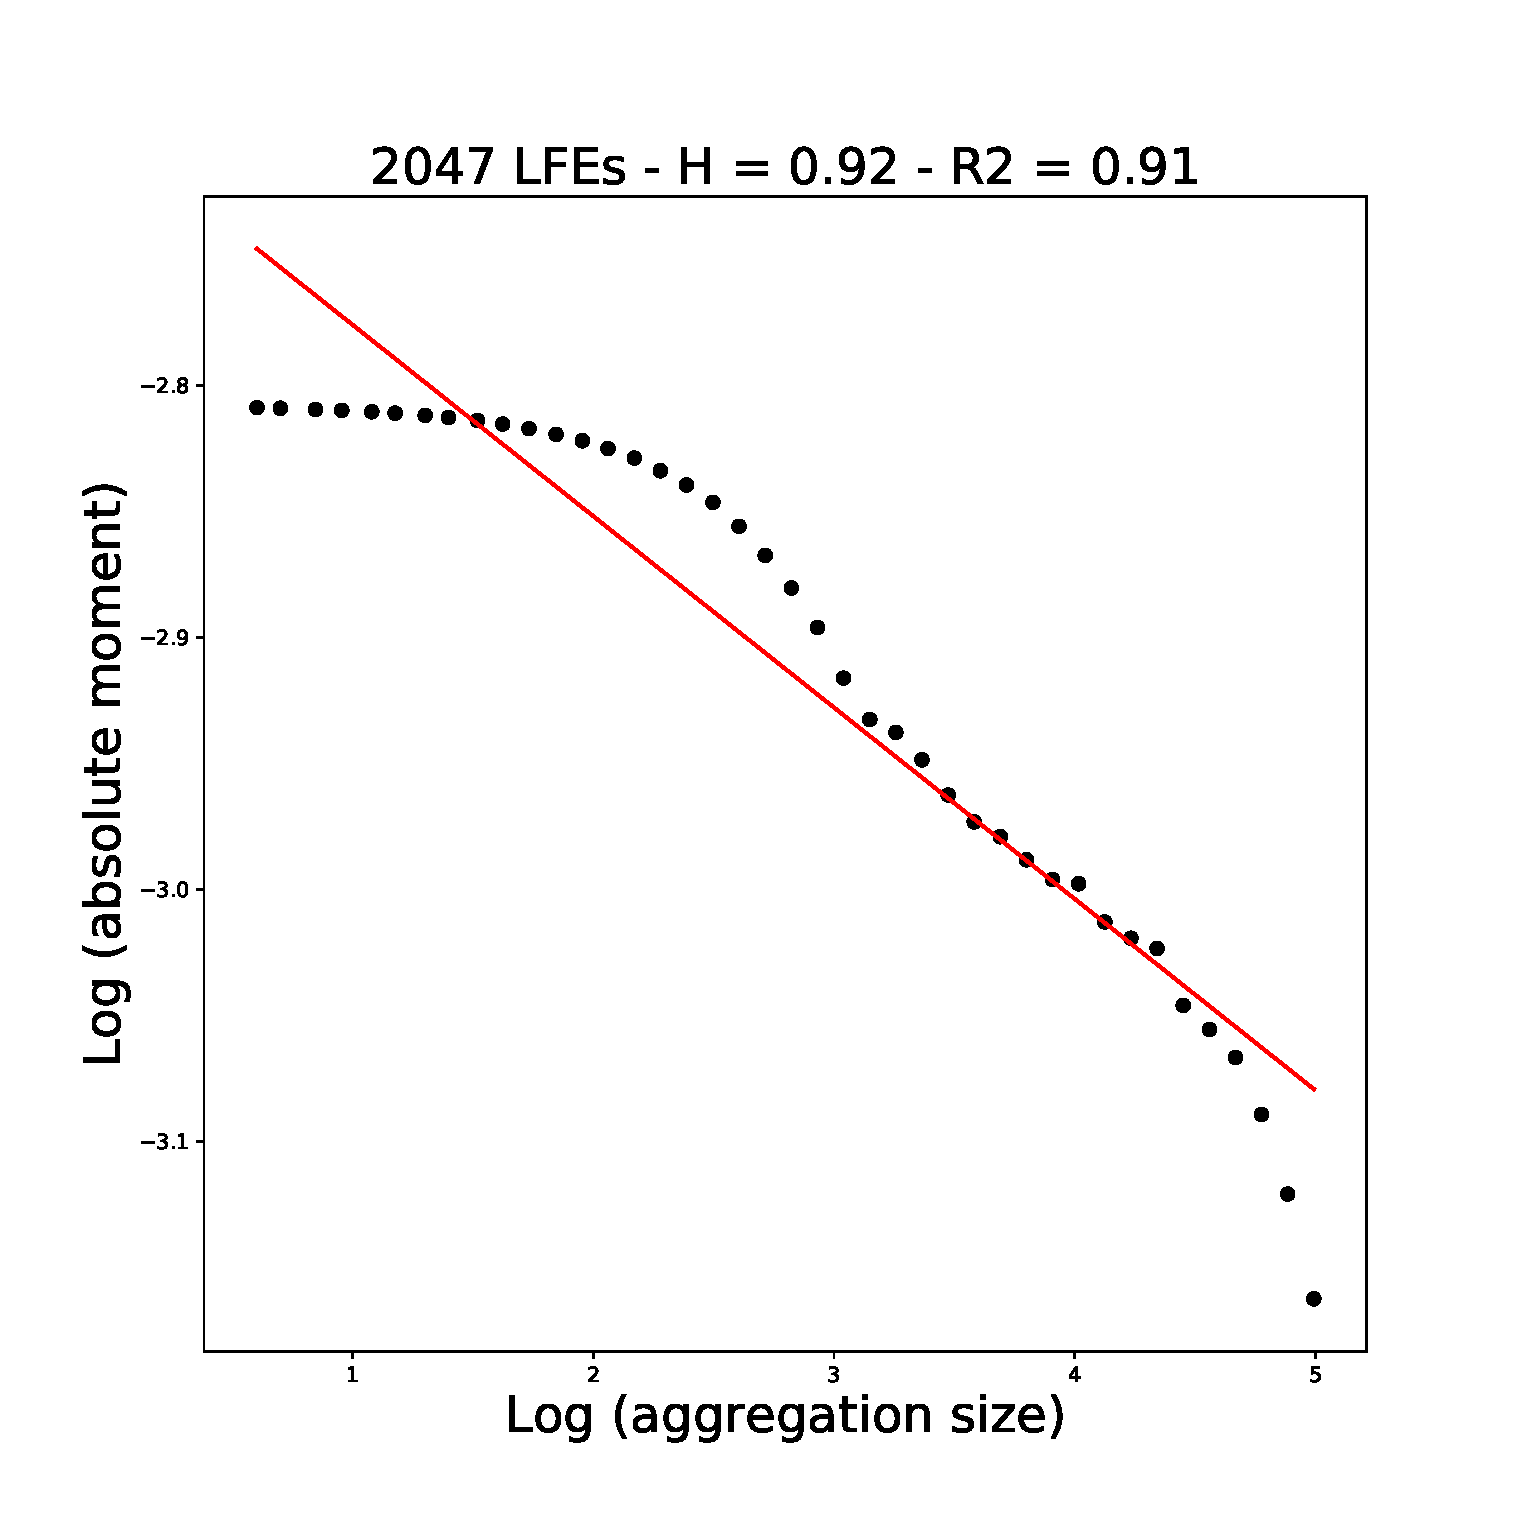
\includegraphics[width=300pt, trim={0cm 0cm 0cm 0cm},clip]{Figures/longrange/absolutevalue.eps}
\captionsetup{type=figure}
\captionof{figure}{Estimation of the Hurst parameter with the absolute value method.}
\end{center}

The sample variance of the time series is:

\begin{equation}
\hat{Var} X^{\left( m \right)} = \frac{m}{N} \sum_{k = 1}^{\frac{N}{m}} \left( X^{\left( m \right)} \left( k \right) - \bar{X} \right) ^2
\end{equation}

and $\hat{Var} X^{\left( m \right)}$ behaves as $m^{2 d - 1}$, where $d$ is the fractional index. The result of the corresponding linear regression can be seen in Figure 8.3.

\begin{center}
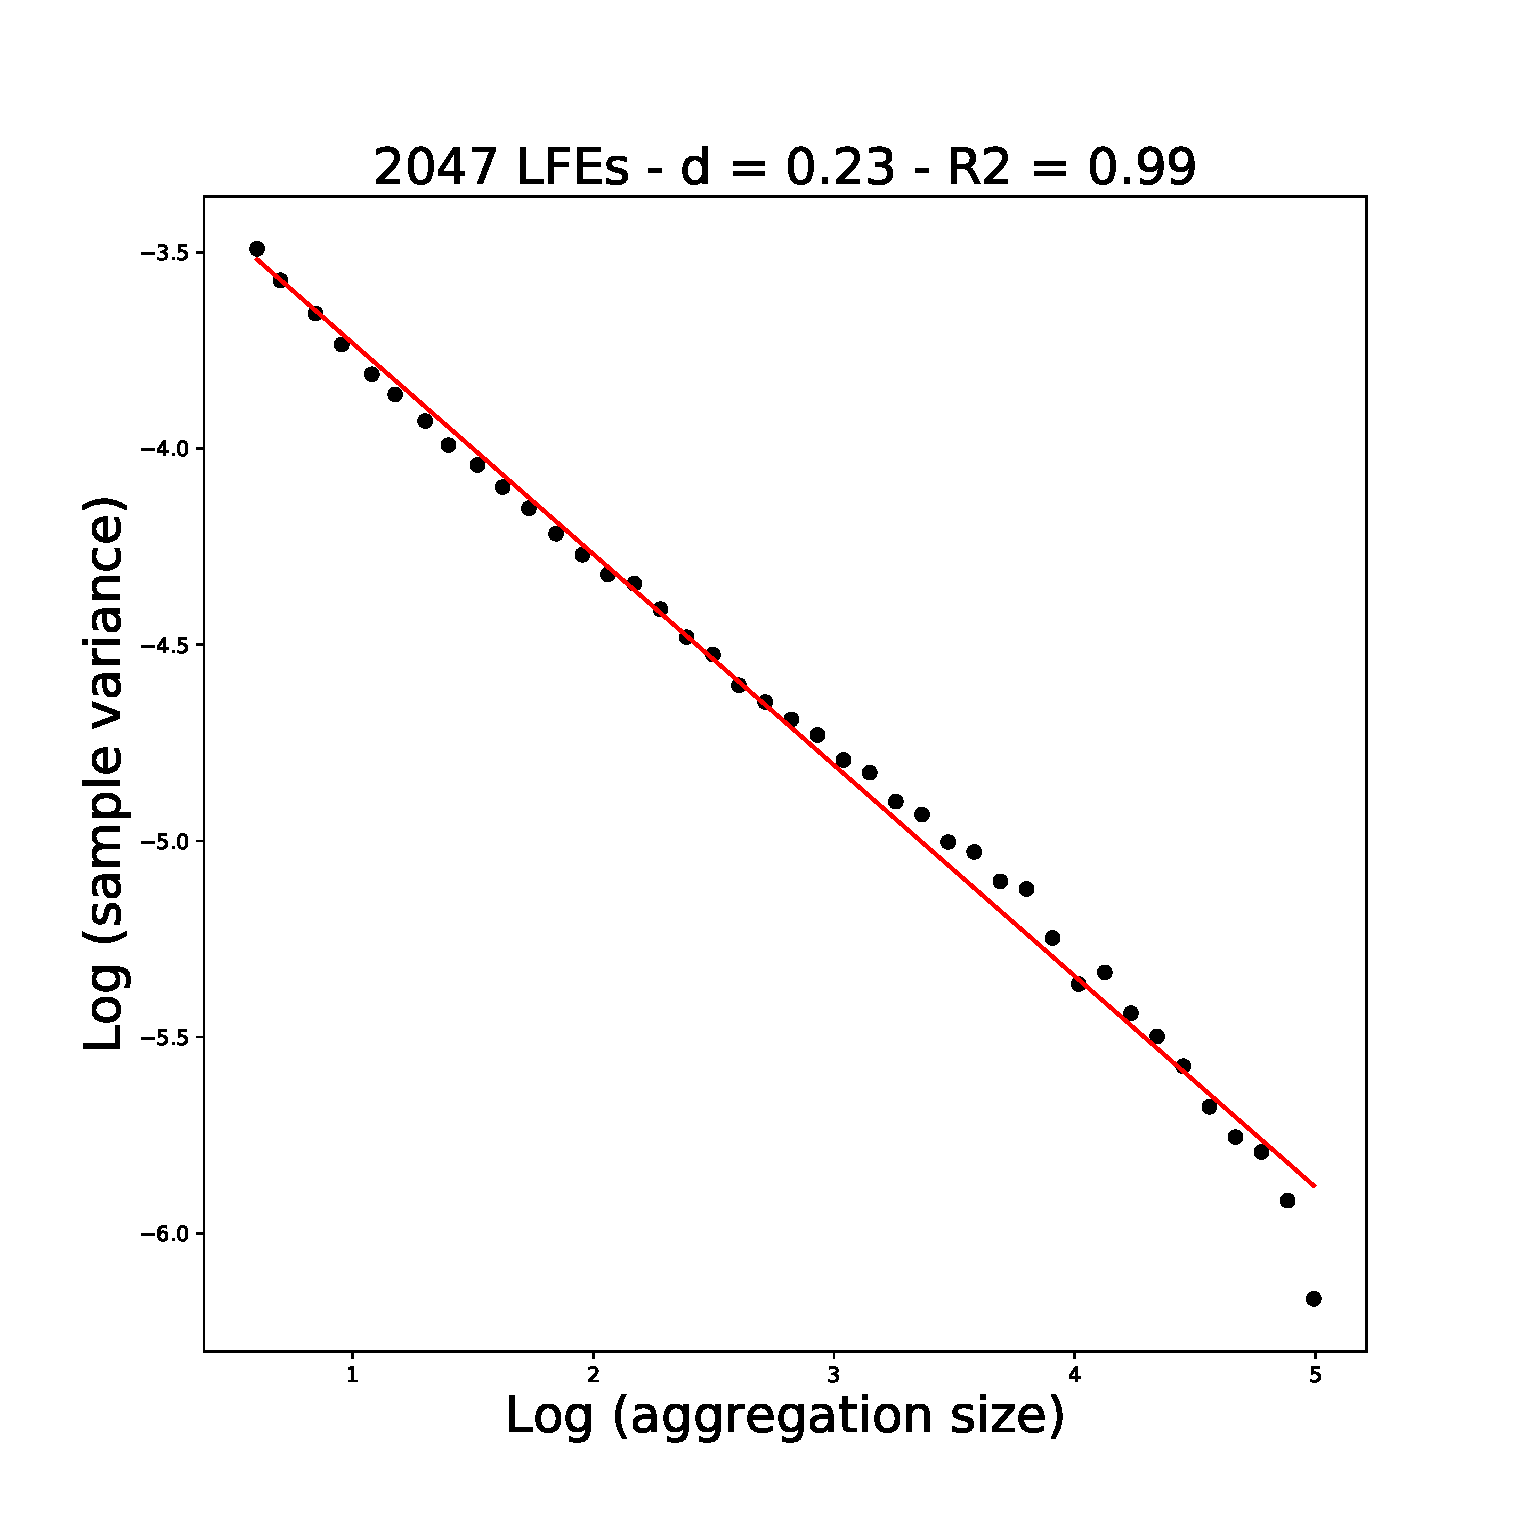
\includegraphics[width=300pt, trim={0cm 0cm 0cm 0cm},clip]{Figures/longrange/variance.eps}
\captionsetup{type=figure}
\captionof{figure}{Estimation of the fractional index with the variance method.}
\end{center}

To define the variance of residuals, we divide the time series into blocks of size $m$. We then compute the partial sums of the time series $Y \left( t \right) = \sum_{i = 1}^{t} X_i$, and fit the partial sums within each block by a least-squares line $a + b t$. The sample variance $\frac{1}{m} \sum_{t = 1}^{m} \left( Y \left( t \right) - a - b t \right) ^2$ is then computed, and its average is proportional to $m^{2 d + 1}$. The result of the corresponding linear regression can be seen in Figure 8.4.

\begin{center}
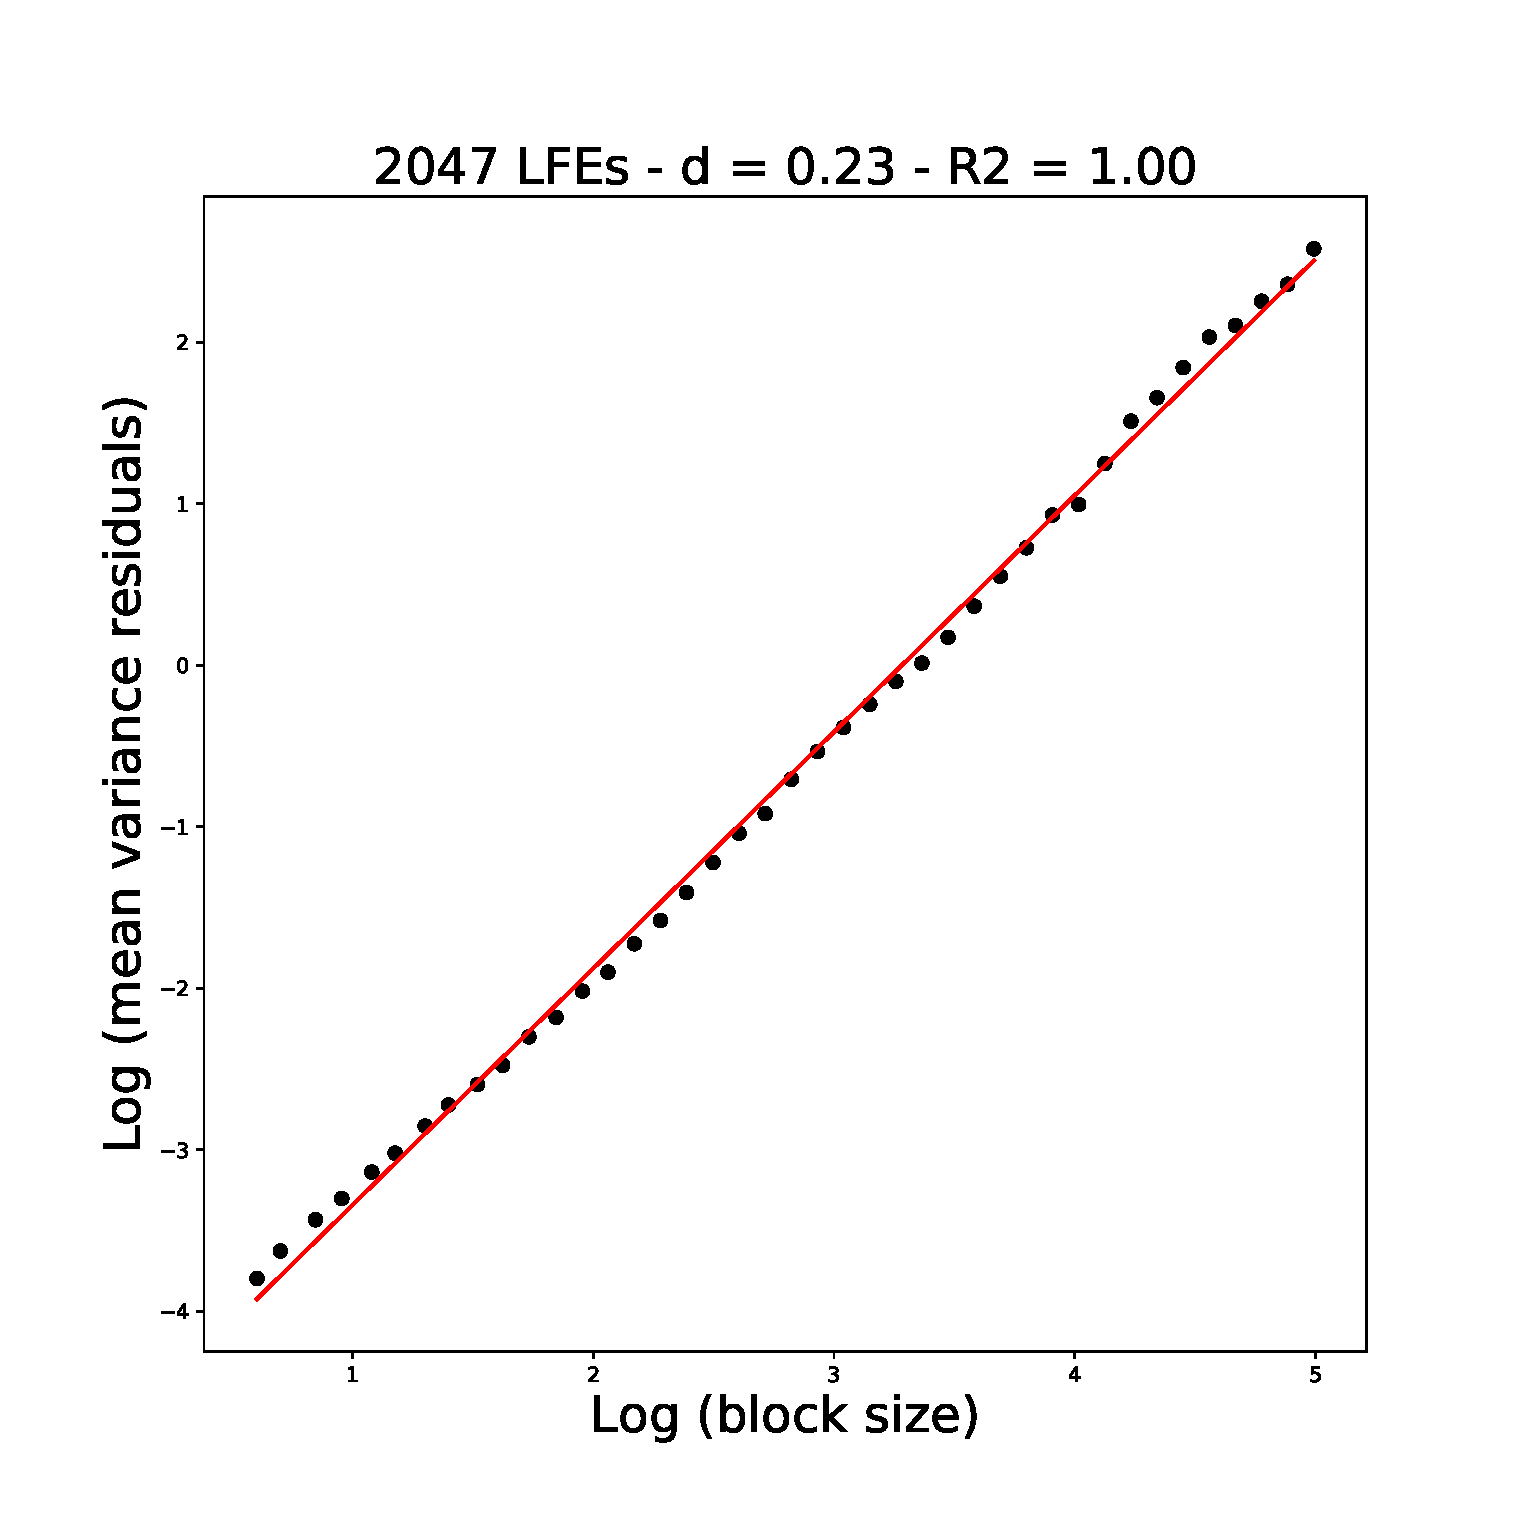
\includegraphics[width=300pt, trim={0cm 0cm 0cm 0cm},clip]{Figures/longrange/varianceresiduals.eps}
\captionsetup{type=figure}
\captionof{figure}{Estimation of the fractional index with the variance of residuals method.}
\end{center}

The $R / S$ statistics is defined by:

\begin{equation}
R \left( t , k \right) = \max_{0 \leq i \leq k} \left[ Y_{t + i} - Y_t - \frac{i}{k} \left( Y_{t + k} - Y_t \right) \right] - \min_{0 \leq i \leq k} \left[ Y_{t + i} - Y_t - \frac{i}{k} \left( Y_{t + k} - Y_t \right) \right]
\end{equation}

\begin{equation}
S \left( t , k \right) = \sqrt{ \frac{1}{k} \sum_{i = t + 1}^{t + k} \left( X_i - \bar{X}_{t , k} \right) ^2 }
\end{equation}

and $R / S = \frac{R \left( t , k \right)}{S \left( t , k \right)}$ behaves as $k^{d + 1 / 2}$. The result of the corresponding linear regression can be seen in Figure 8.5.

\begin{center}
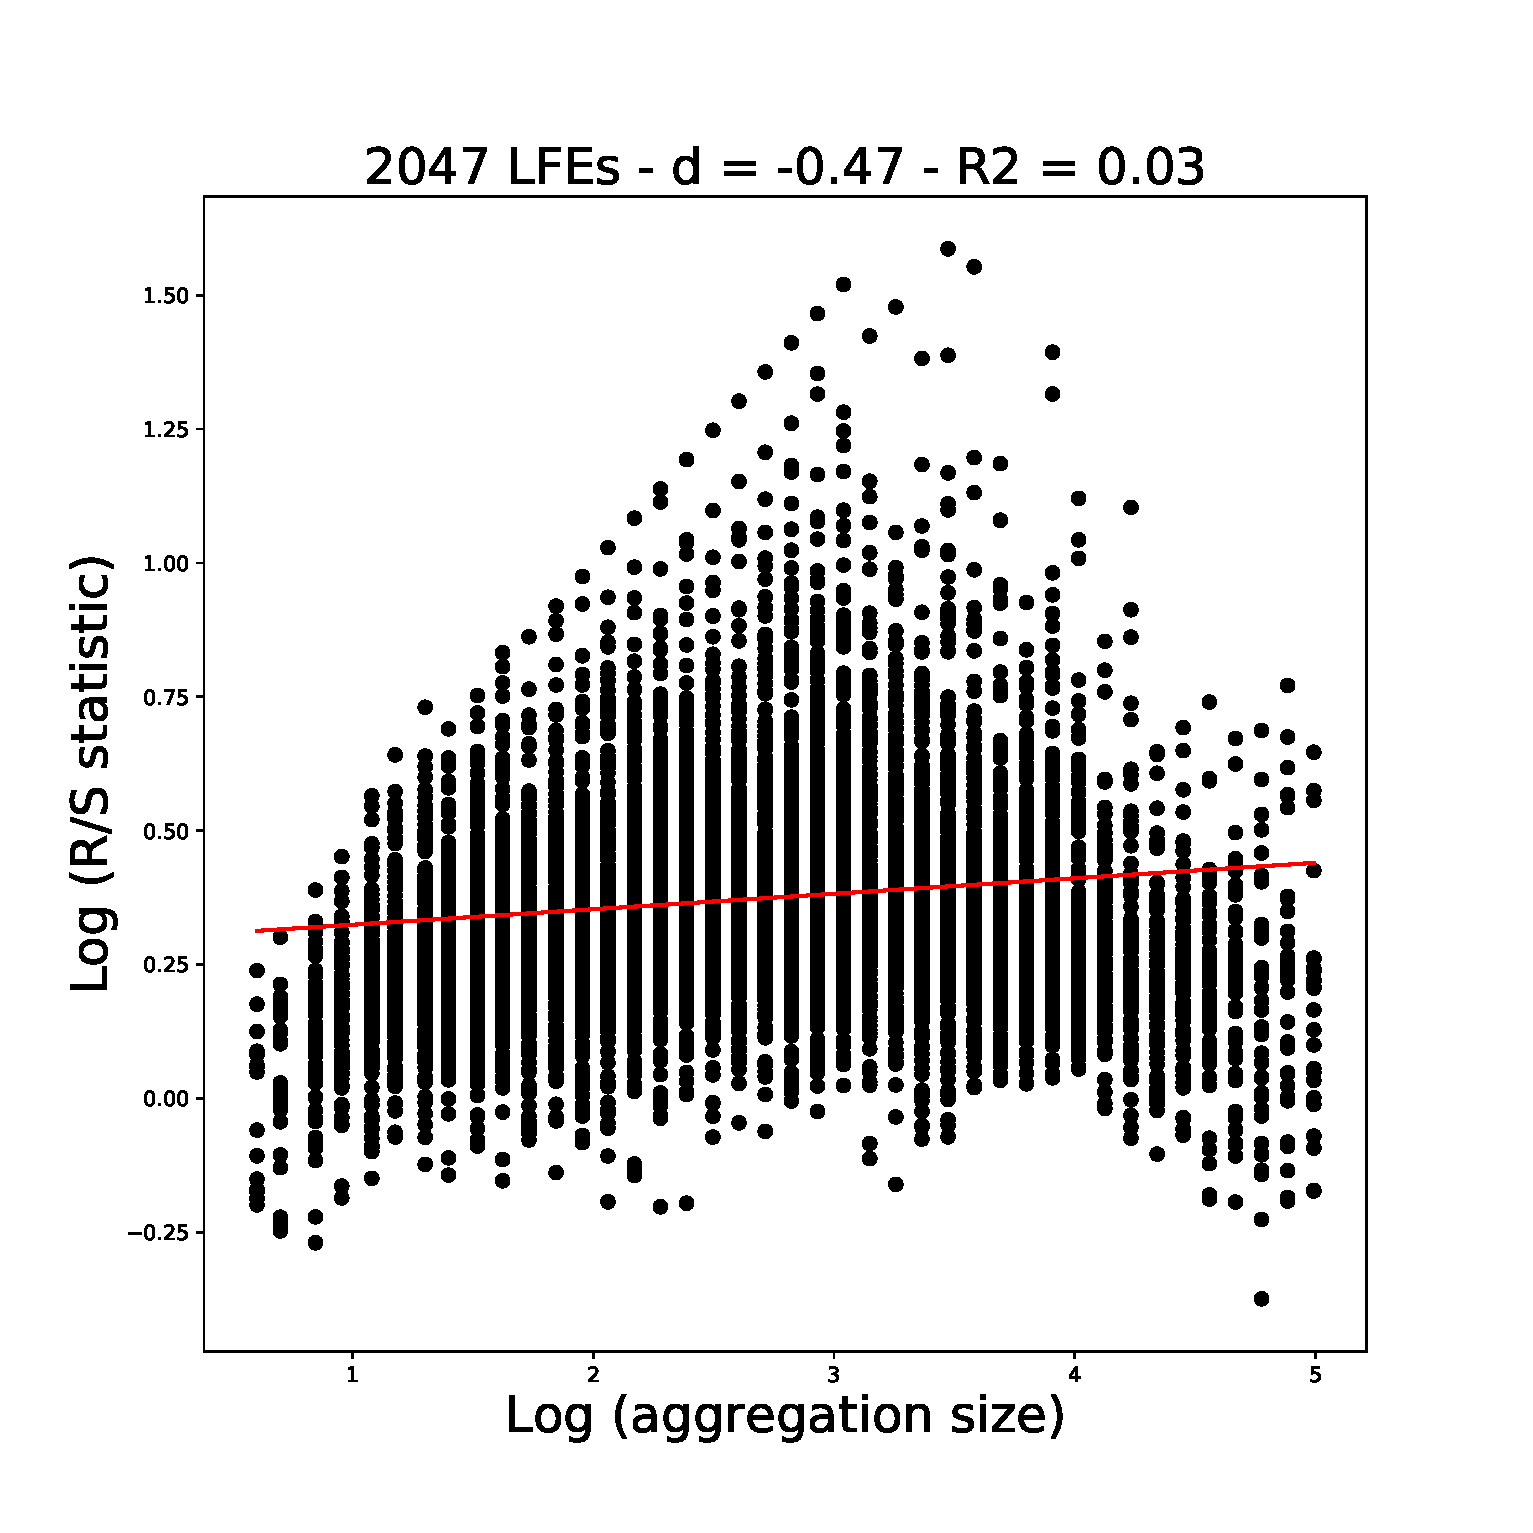
\includegraphics[width=300pt, trim={0cm 0cm 0cm 0cm},clip]{Figures/longrange/RS.eps}
\captionsetup{type=figure}
\captionof{figure}{Estimation of the fractional index with the R/S method.}
\end{center}

The periodogram  is defined as:

\begin{equation}
I \left( \nu \right) = \frac{1}{2 \pi N} \left| \sum_{j = 1}^N X \left( j \right) e^{i j \nu} \right| ^2
\end{equation}

and $I \left( \nu \right)$ behaves as $\left| \nu \right| ^{- 2 d}$ close to the origin. The result of the corresponding linear regression can be seen in Figure 8.6.

\begin{center}
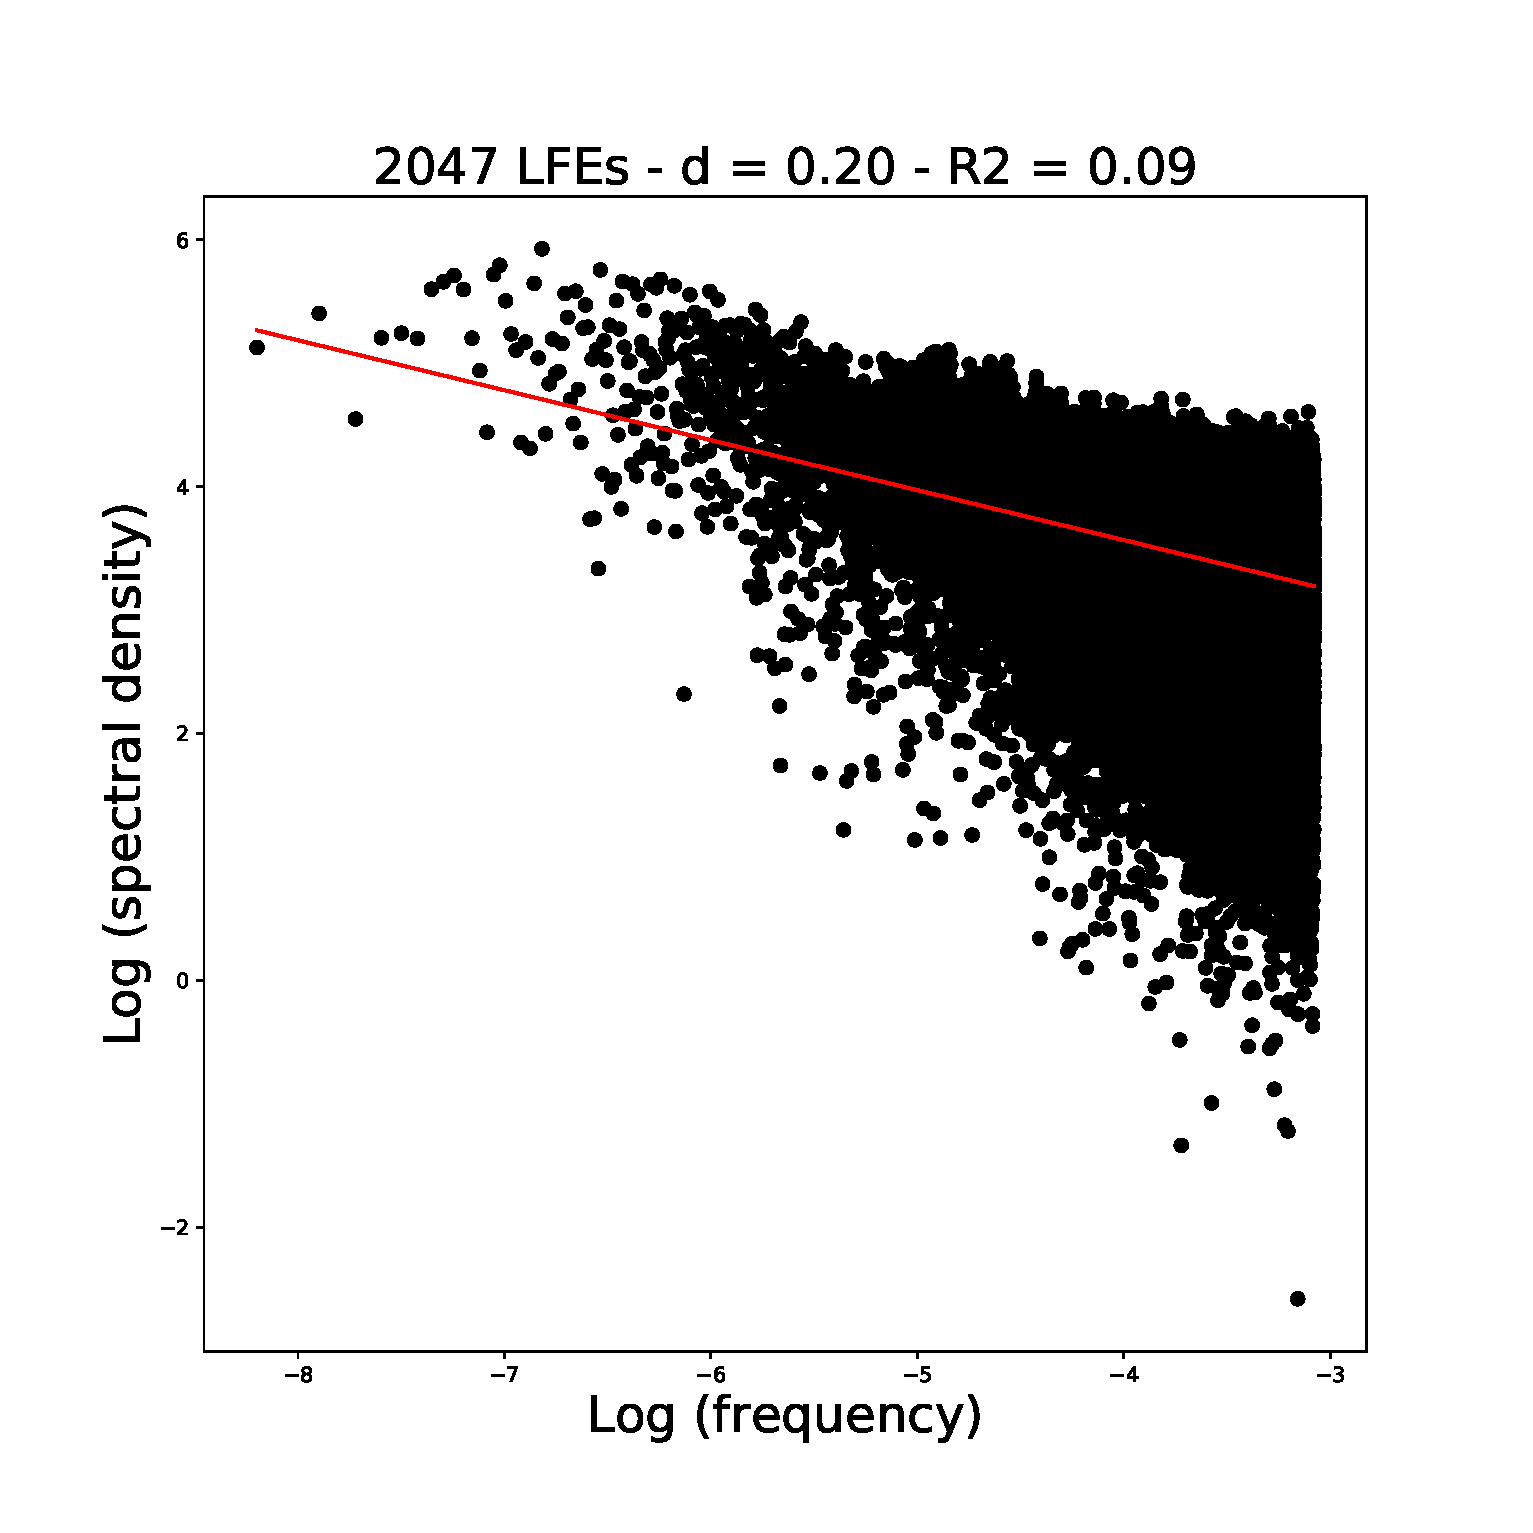
\includegraphics[width=300pt, trim={0cm 0cm 0cm 0cm},clip]{Figures/longrange/periodogram.eps}
\captionsetup{type=figure}
\captionof{figure}{Estimation of the fractional index with the periodogram method.}
\end{center}

Frank, WB ; Shapiro, NM ; Husker, AL ; Kostoglodov, V ; Gusev, AA ; Campillo, M. The evolving interaction of low-frequency earthquakes during transient slip. Science Advances, 2016 Apr, Vol.2(4).

Sweet, Justin R. ; Creager, Kenneth C. ; Houston, Heidi. A family of repeating low‐frequency earthquakes at the downdip edge of tremor and slip. Geochemistry, Geophysics, Geosystems, September 2014, Vol.15(9), pp.3713-3721.

Murad S. Taqqu and Vadim Teverovsky. On estimating the intensity of long-range dependence in finite and infinite variance time series. In: A practical guide to heavy tails : statistical techniques and applications. Robert J. Adler; Raisa E. Feldman, 1958-; Murad S. Taqqu; 1998 Boston : Birkhäuser.

\end{document}
